\documentclass[12pt]{book} 

\usepackage{amsmath}
\usepackage{graphicx}
\usepackage{import}
\usepackage{amsfonts}
\usepackage{booktabs}

\setlength{\parindent}{0em}  % sets auto indent at new paragraph to none

\newcommand{\incfig}[1]{%
    \import{./figures/}{#1.pdf_tex}
}

\title{\coursetitle\linebreak\lecturename}
\author{\\Cain Susko\\ 
           \\ \\ \\
      Queen's University 
    \\School of Computing\\} 

%=-=-=-=-=-title-=-=-=-=-=%
\newcommand{\lecturename}{Machine Representation of Programs: Control}
\newcommand{\coursetitle}{Computer Architecture}
%=-=-=-=-=-#####-=-=-=-=-=%

\begin{document}
\begin{titlepage}
        \maketitle
\end{titlepage}


\section*{Conditional Branches}
Equivalent to the `if' statement that computers use.
There are many types of conditional branches:

\paragraph{Jumps}
Known as $jX$ instructions, these make the program jump to different parts of code depending on condition codes.
 \begin{figure}[h]
        \centering
        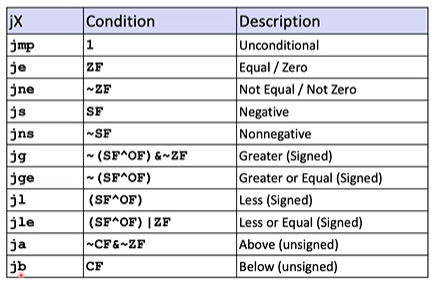
\includegraphics{./figures/jx}
\end{figure}

An example of an `Old Sytle' Conditional Branch
\begin{figure}[h]
        \centering
        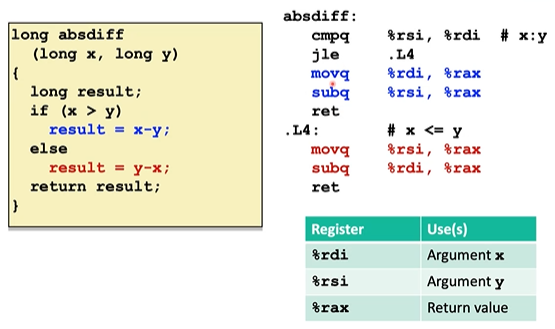
\includegraphics[scale = 0.7]{./figures/jxEx}
\end{figure}
\pagebreak

This is old style because The GoTo Function was implemented in C which allows for the following:
\begin{figure}[h]
        \centering
        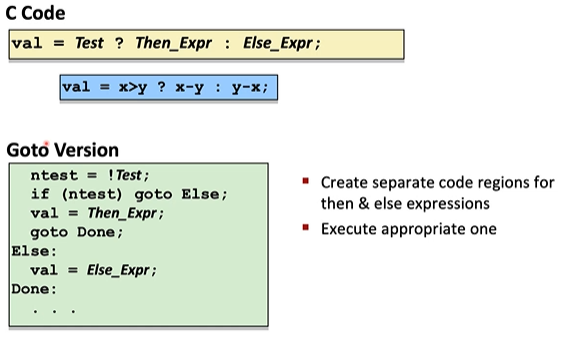
\includegraphics[scale = 0.5]{./figures/gotoEx}
        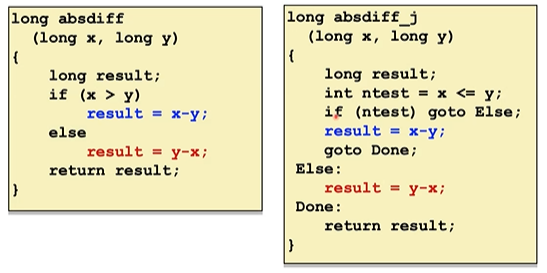
\includegraphics[scale = 0.6]{./figures/gotoEx2}
\end{figure}

The above programs are the old C code on the left compared to the New GoTo C code on the right. This makes the C code more
functionally similar to the Assembly code. But because it is a hardcoded jump rather than a branch (like an if statement)
the computer cannot pipeline (predict the program) efficiently which is a drain on performance.
\pagebreak

\section*{Conditional Move}


The following is an example of a Conditional Move (which is preferable to Goto):
\begin{figure}[h]
        \centering
        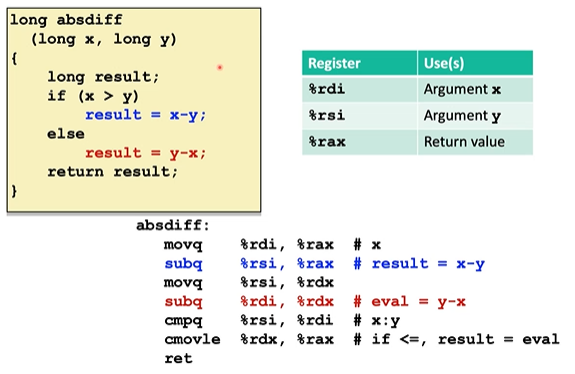
\includegraphics[scale = 0.51]{./figures/ifThenMoveEx}
\end{figure}

Note that this is a different representation of the example on page 2 of this note which uses conditional moves rather than
jumps.

\paragraph{Bad Cases}
There are a few cases where a conditional jump is not good to use. First, if the computation for the if statement is very
complex the computational benefit for using a conditional statement is outweighed by the computational load used to 
compute the conditions.
\[
\texttt{val = Test(x) ? HardComp1(x) : HardComp2(x);}
.\] 
When a computation is risky, a conditional branch may cause undefined or undesirable behaviour.
\[
\texttt{val = p ? *p : 0;}
.\] 

Finally, if the computations in each branch have `side effects' then a conditional move should not be used.
\[
\texttt{val = x > 0 ? x*=7 : x+=3;}
.\] 
This is because both of the values get computed and causes more computational resources to be used.

\subsection*{Conditional Branch - if statement summary}
we now know that we can use two different methods of implementing $if$ statements in code. They are:
\begin{itemize}
        \item conditional Jumps
        \item conditional Moves
\end{itemize}

\section*{Loops}
Loops can be implemented with simply with an inf statement. in C code, there are 3 categories of loops. 
\subsection*{Do While}
The first is the 
`Do While' loop which does something while it is true. In C code this can be represented with either an $if$ statement or
using the Goto function:
\begin{figure}[h]
        \centering
        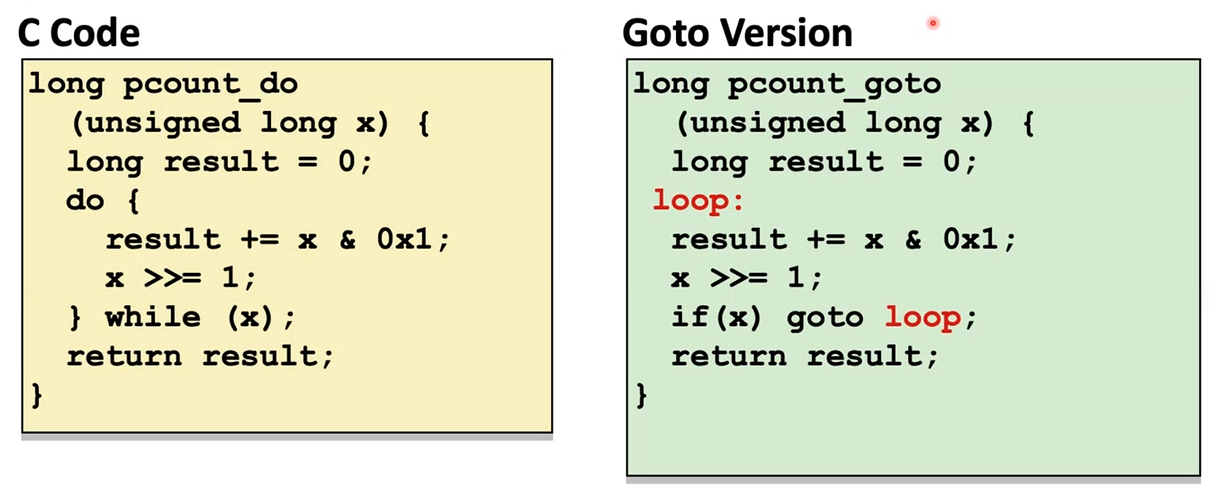
\includegraphics[scale = 0.4]{./figures/doWhile}
\end{figure}

These are both equivalent; however the goto version makes the code unnecissarily complicated. The assembly code for this
loop is:
\pagebreak


\begin{figure}[h]
        \centering
        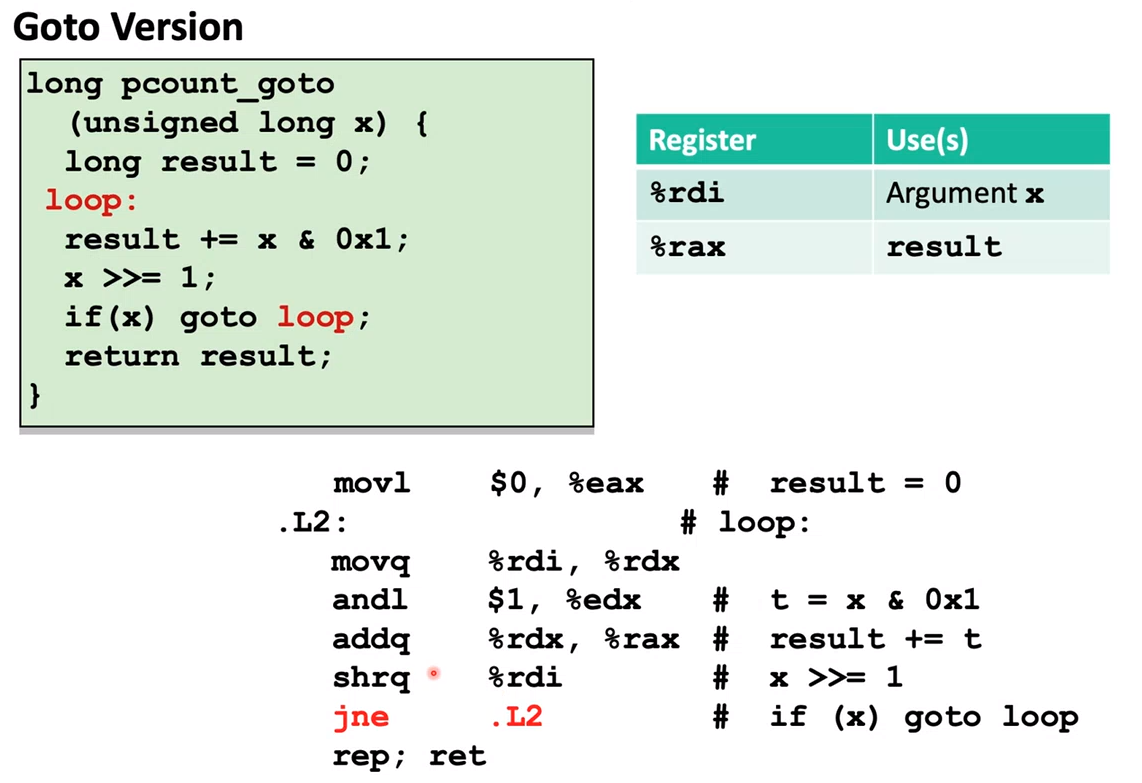
\includegraphics[scale = 0.3]{./figures/doWhileAsmbly}
\end{figure}


Below is the general form for \textbf{do while} loops in C:
\begin{figure}[h]
        \centering
        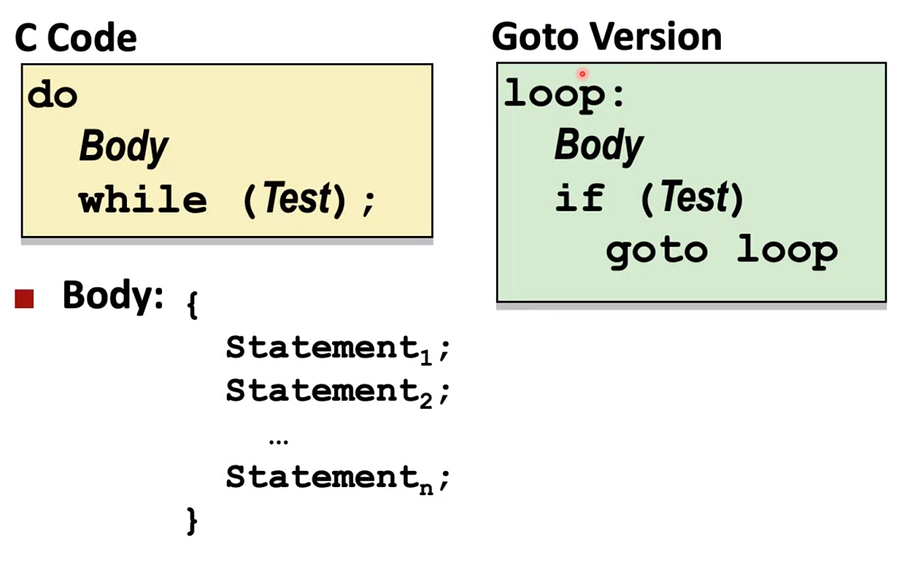
\includegraphics[scale = 0.4]{./figures/doWhileGeneral}
\end{figure}
\pagebreak

\subsection*{While}
While loops are similar to do-while for obvious reasons. The general form for a \textbf{while} loop in C is:
\begin{figure}[h]
        \centering
        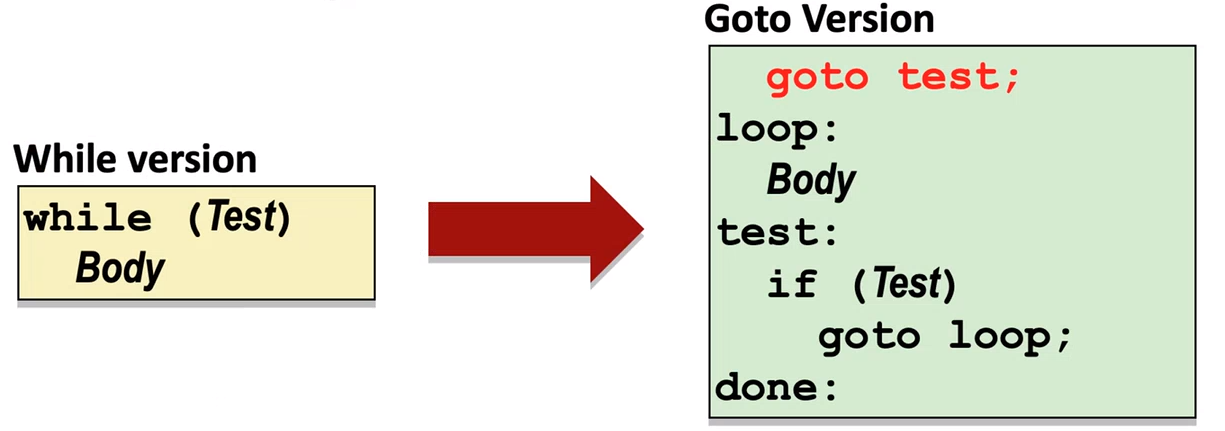
\includegraphics[scale = 0.4]{./figures/whileGeneral}
\end{figure}

We can also generalize the while loop in terms of the do while loop like so:
\begin{figure}[h]
        \centering
        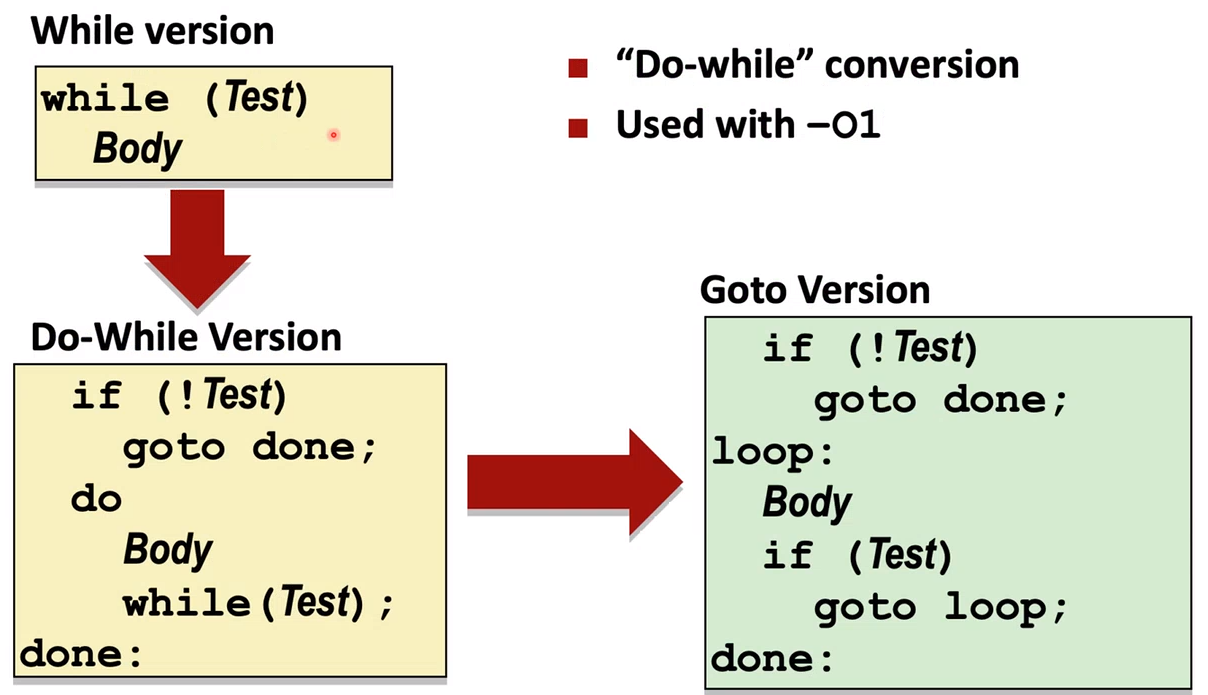
\includegraphics[scale = 0.4]{./figures/whileGeneral2}
\end{figure}
\pagebreak


Using this generalization we can reform a while loop to be a `do while' for loop:
\begin{figure}[h]
        \centering
        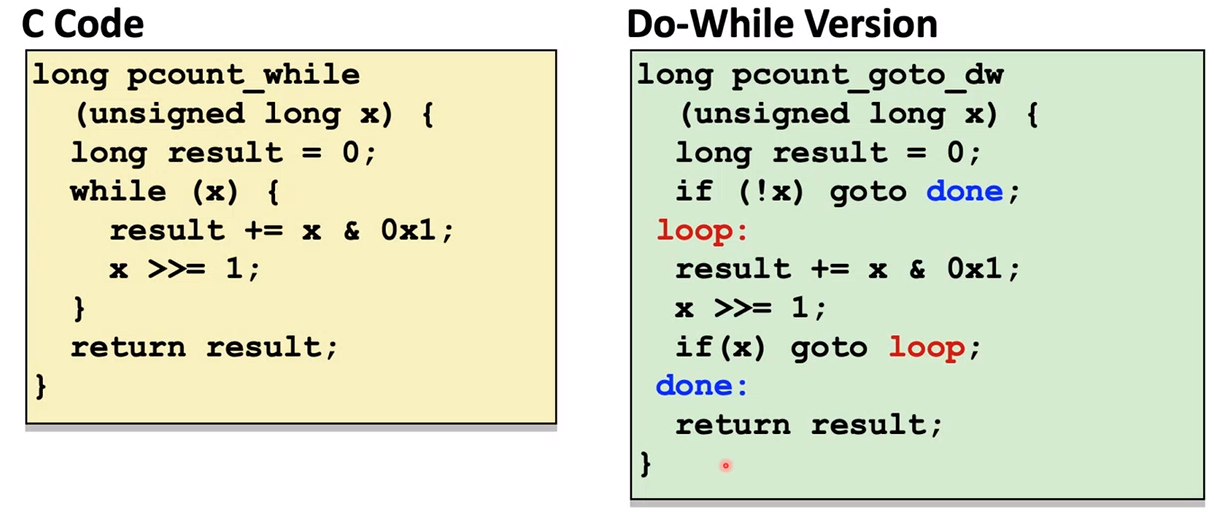
\includegraphics[scale = 0.4]{./figures/whileDoWhile}
\end{figure}

\subsection*{For}
The for loop has the general form in C (and most other languages) is :
\[
\texttt{for (i = InitVal; i < Test; i++)}
.\] 

To convert a for loop to a `for while' loop the general form is:
\begin{figure}[h]
        \centering
        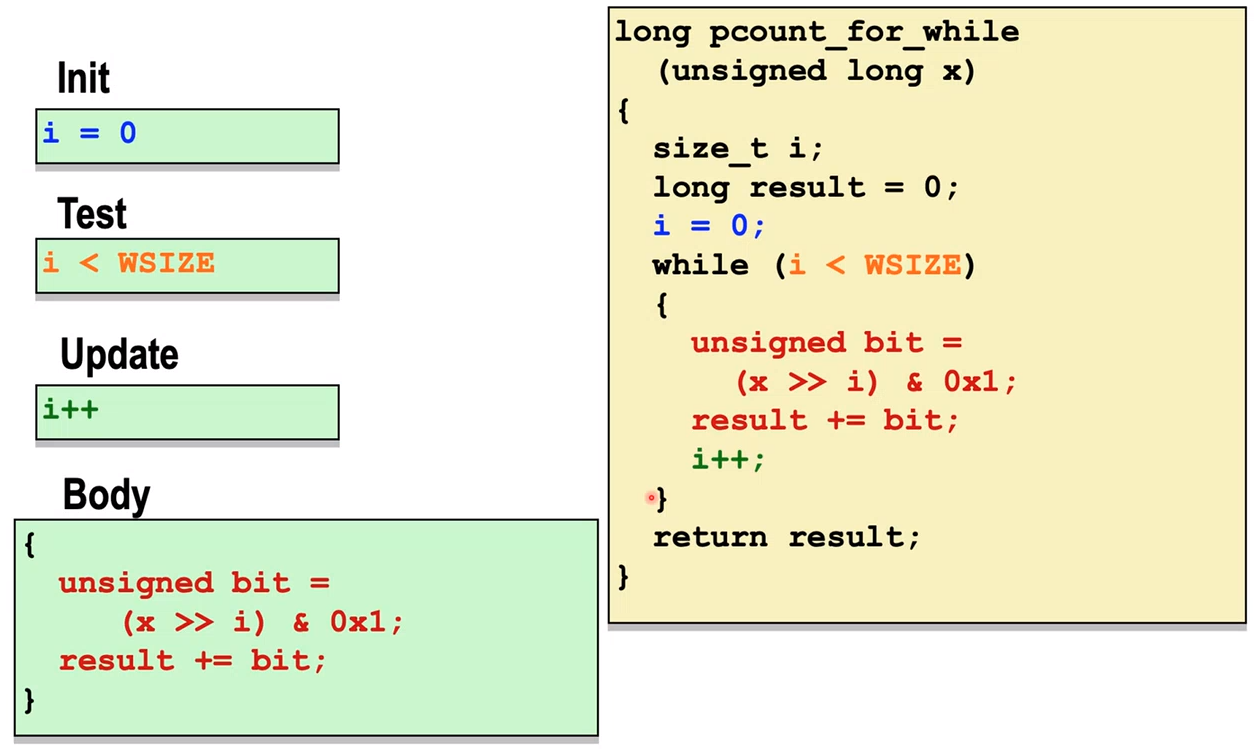
\includegraphics[scale = 0.2]{./figures/forWhile}
\end{figure}
\pagebreak

We can also convert from for loop to a do while loop like so:
\begin{figure}[h]
        \centering
        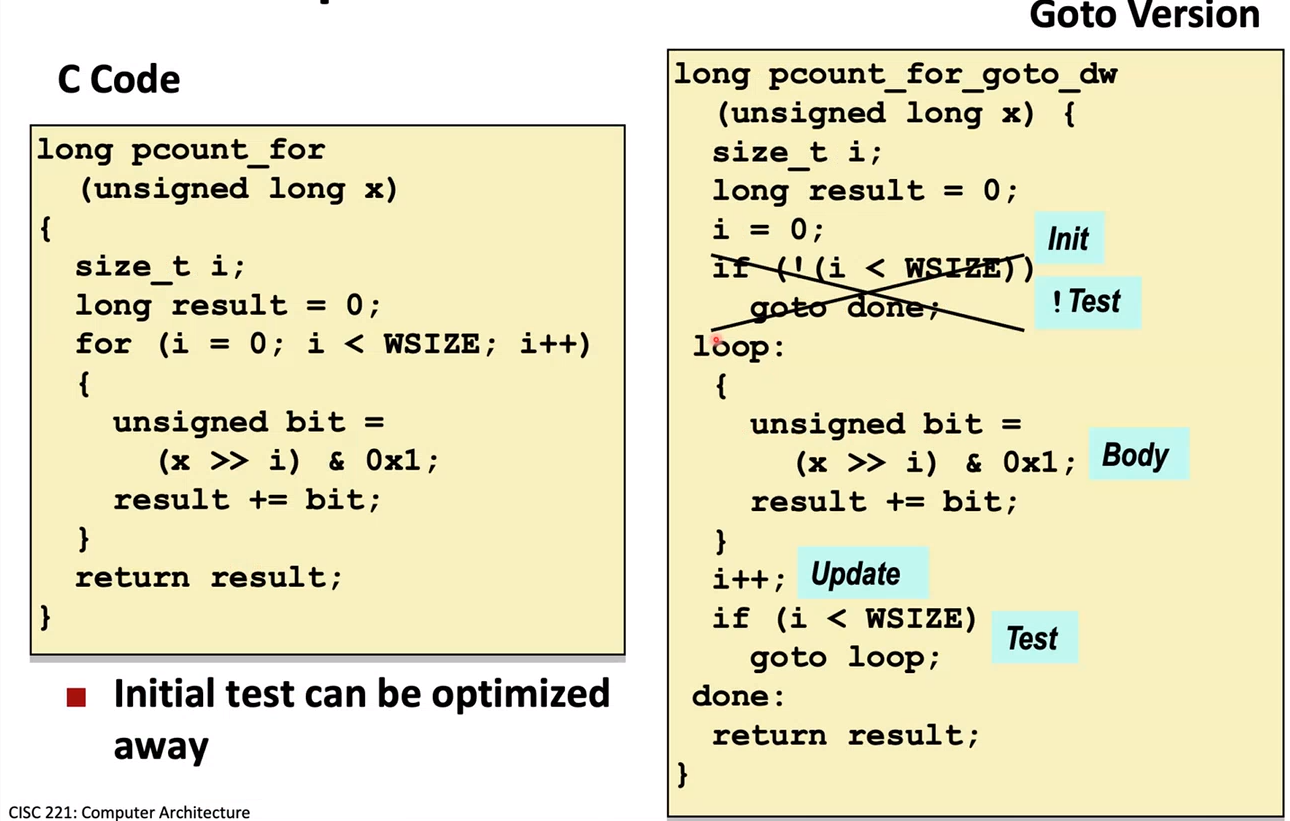
\includegraphics[scale = 0.3]{./figures/forDoWhile}
\end{figure}

\section*{Switch Statement}
The final control structure we will cover is the switch statement.

\begin{figure}[h]
        \centering
        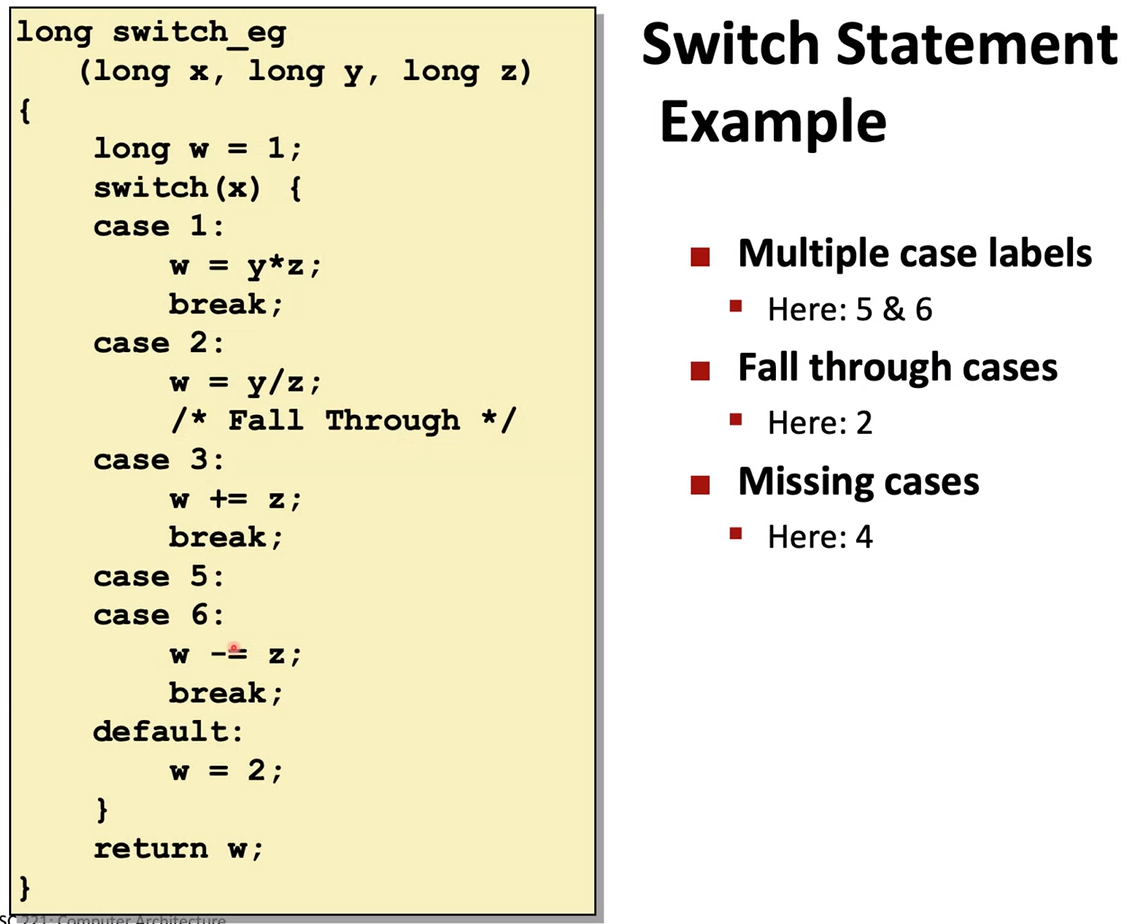
\includegraphics[scale = 0.3]{./figures/switch}
\end{figure}

This structure is acheived by using a Jump Table with different identifiers. This is done like so:
\begin{figure}
        \centering
        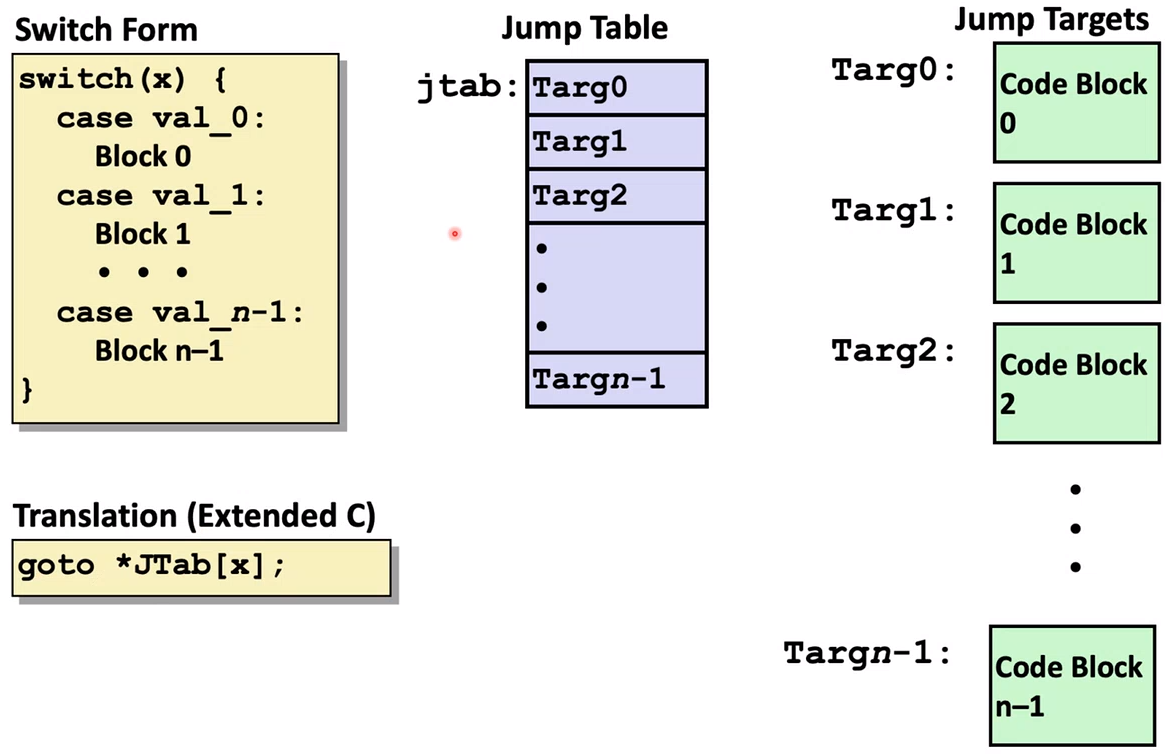
\includegraphics[scale = 0.4]{./figures/jumpTable}
\end{figure}

Showing this with the example from before:
\begin{figure}[h]
        \centering
        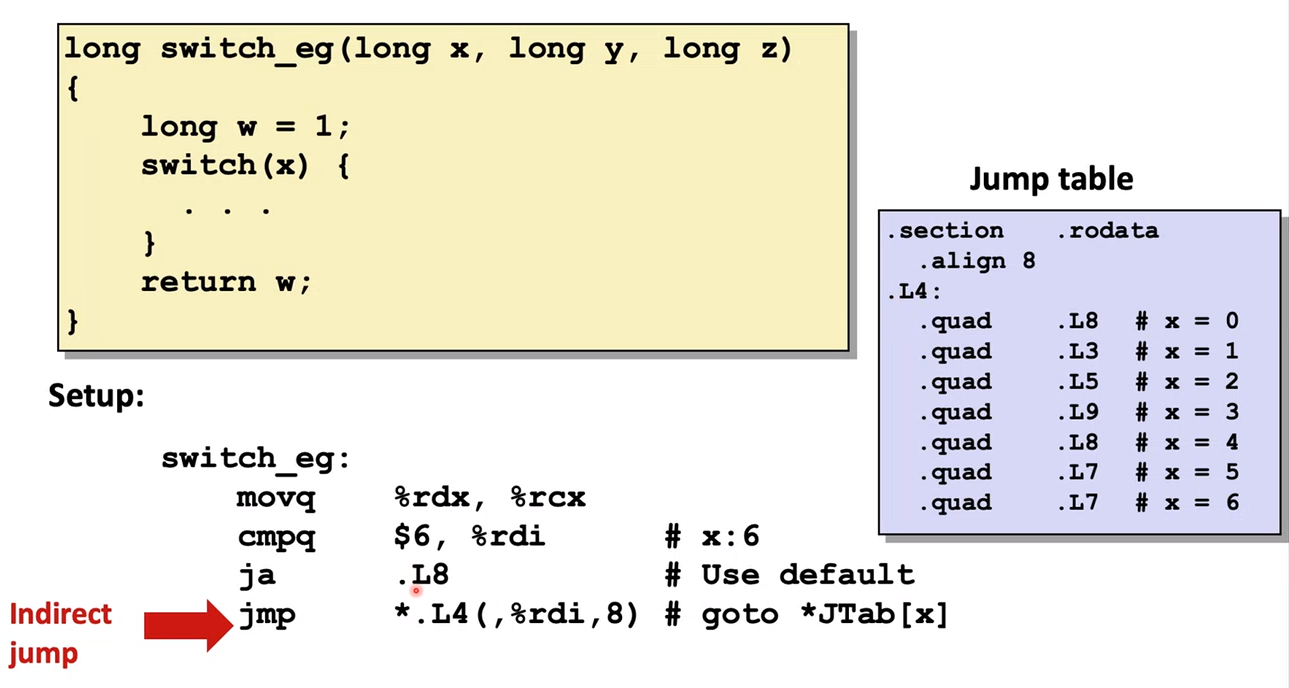
\includegraphics[scale = 0.3]{./figures/switchEx}
\end{figure}

And thus, the general setup in assembly for a switch statement is:
\pagebreak

\begin{figure}[h]
        \centering
        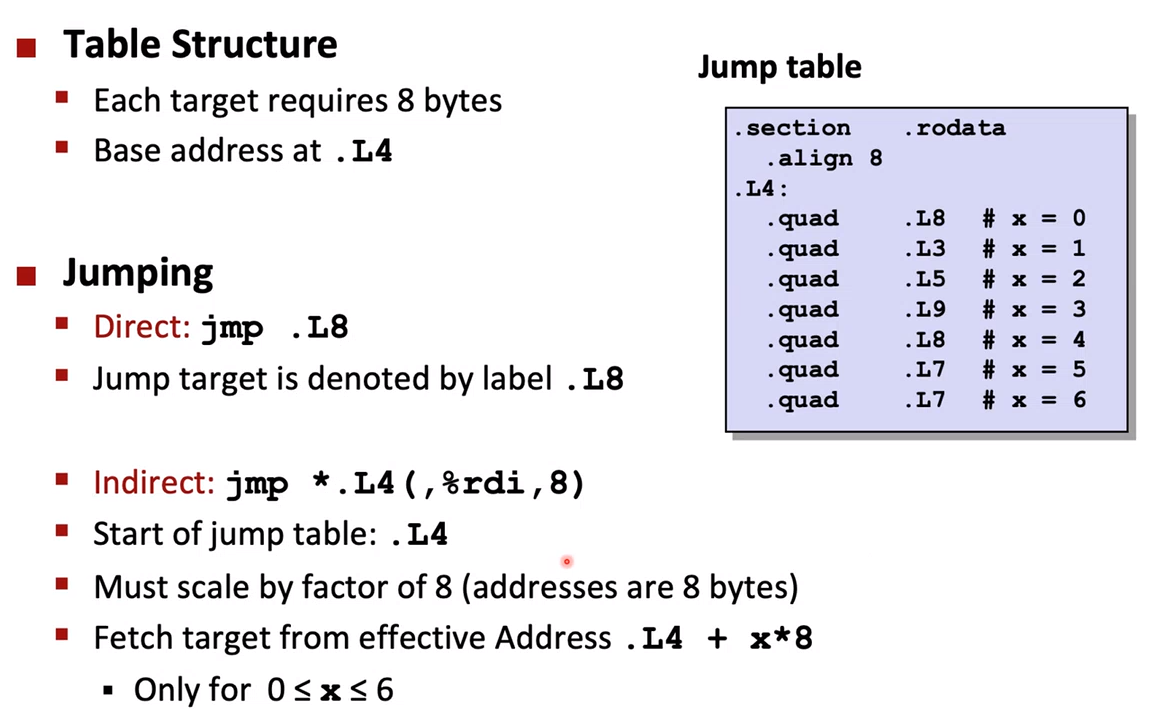
\includegraphics[scale = 0.3]{./figures/switchStruct}
        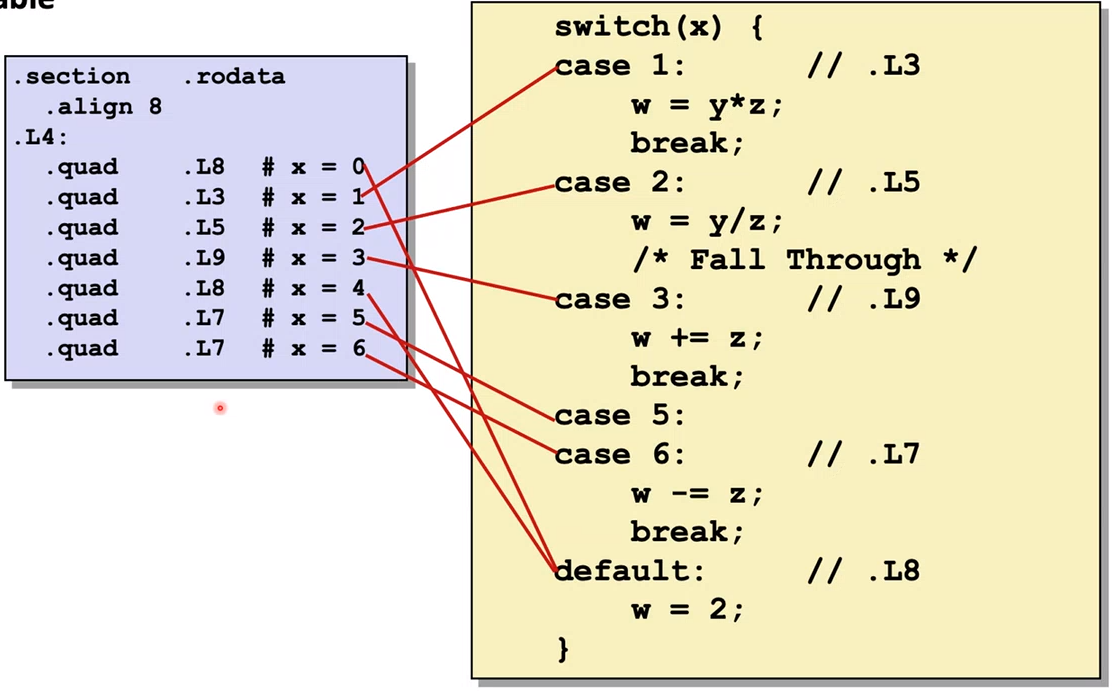
\includegraphics[scale = 0.3]{./figures/switchEx2}
\end{figure}

\section*{Summary}
In C we can implement Control by using:
\begin{itemize}
        \item if-then-else
        \item do-while
        \item while, for
        \item switch
\end{itemize}

Within the Assembler there are 4 ways of achieveing these:
\begin{itemize}
        \item conditional Jump
        \item conditional Move
        \item indirect jump (via jump table)
        \item compiler generates code sequence to implement more complex control
\end{itemize}

Some standard techniques for operating on control structures are:
\begin{itemize}
        \item converting loops to do-while or `lump-to-middle' form
        \item large switch statements use jump tables
        \item sparse switch statements may use desision trees (if-elseif-elseif-\ldots)
\end{itemize}

\end{document}

